\documentclass[10pt,a4paper,twocolumn]{article}

\usepackage[T1]{fontenc}
\usepackage[utf8]{inputenc}
\usepackage{lmodern}
\usepackage[margin=1.7cm,columnsep=0.7cm]{geometry}
\usepackage{amsmath}
\usepackage{booktabs}
\usepackage{tikz}
\usepackage{caption}
\usepackage{microtype}
\usepackage{enumitem}
\usepackage[round,sort]{natbib}
\usepackage[hidelinks]{hyperref}
\usepackage{xurl}
\usepackage{titlesec}

\captionsetup{font=small,labelfont=bf}
\setlist{nosep,leftmargin=1.2em}
\titleformat{\section}{\normalfont\large\bfseries}{}{0pt}{}
\titlespacing*{\section}{0pt}{8pt}{3pt}
\setlength{\parskip}{3pt}
\setlength{\parindent}{0pt}
\pagestyle{empty}
% Generated by make_tables.py; do not edit.
\newcommand{\nTestRows}{84{,}200}
\newcommand{\maeModel}{0.996}
\newcommand{\maeForm}{1.052}
\newcommand{\corrModel}{0.575}
\newcommand{\corrForm}{0.493}
\newcommand{\capModel}{6.61}
\newcommand{\capElite}{8.20}
\newcommand{\capPremium}{5.16}
\newcommand{\capForm}{5.25}
\newcommand{\capBest}{17.79}
\newcommand{\capRegret}{11.18}
\newcommand{\gapElite}{1.59}
\newcommand{\vsElite}{$-1.59$ ($-2.50$ to $-0.73$)}
\newcommand{\vsEliteMean}{$-1.59$}
\newcommand{\vsEliteLow}{$-2.50$}
\newcommand{\vsEliteHigh}{$-0.73$}
\newcommand{\vsElitePlot}{-2.500,-1.588,-0.728}
\newcommand{\vsPremium}{$+1.46$ ($+0.42$ to $+2.49$)}
\newcommand{\vsPremiumMean}{$+1.46$}
\newcommand{\vsPremiumLow}{$+0.42$}
\newcommand{\vsPremiumHigh}{$+2.49$}
\newcommand{\vsPremiumPlot}{0.421,1.456,2.491}
\newcommand{\vsForm}{$+1.37$ ($+0.22$ to $+2.48$)}
\newcommand{\vsFormMean}{$+1.37$}
\newcommand{\vsFormLow}{$+0.22$}
\newcommand{\vsFormHigh}{$+2.48$}
\newcommand{\vsFormPlot}{0.219,1.368,2.483}
\newcommand{\capModelA}{5.89}
\newcommand{\capEliteA}{7.29}
\newcommand{\capPremiumA}{5.92}
\newcommand{\capFormA}{4.68}
\newcommand{\capModelB}{9.11}
\newcommand{\capEliteB}{10.13}
\newcommand{\capPremiumB}{5.26}
\newcommand{\capFormB}{6.71}
\newcommand{\capModelC}{4.84}
\newcommand{\capEliteC}{7.18}
\newcommand{\capPremiumC}{4.29}
\newcommand{\capFormC}{4.34}
\newcommand{\nSquadWeeks}{11{,}400}
\newcommand{\lineModel}{66.00}
\newcommand{\lineManager}{68.29}
\newcommand{\lineForm}{63.76}
\newcommand{\lineVsManager}{$-2.29$ ($-3.04$ to $-1.58$)}
\newcommand{\lineVsManagerPlot}{-3.045,-2.288,-1.578}
\newcommand{\lineVsForm}{$+2.25$ ($+1.16$ to $+3.35$)}
\newcommand{\lineVsFormPlot}{1.162,2.248,3.348}
\newcommand{\iterMin}{70}
\newcommand{\iterMedian}{114.5}
\newcommand{\iterMax}{175}
\newcommand{\acSeasonMin}{$-0.23$}
\newcommand{\acSeasonMax}{$+0.28$}
\newcommand{\sdMin}{4.9}
\newcommand{\sdMax}{6.6}
\newcommand{\rhoModel}{0.71}
\newcommand{\rhoForm}{0.69}
\newcommand{\rhoReg}{0.68}
\newcommand{\maeReg}{1.046}
\newcommand{\maeFormScaled}{1.053}
\newcommand{\rhoCandModel}{0.31}
\newcommand{\rhoCandForm}{0.21}
\newcommand{\rhoCandReg}{0.28}
\newcommand{\maeGainFormScaled}{$+0.057$ ($+0.048$ to $+0.066$)}
\newcommand{\maeGainReg}{$+0.048$ ($+0.041$ to $+0.056$)}
\newcommand{\calSlope}{0.97}
\newcommand{\calIntercept}{0.01}
\newcommand{\nCandRows}{20{,}400}
\newcommand{\capFormScaled}{6.18}
\newcommand{\vsFormScaled}{$+0.43$ ($-0.81$ to $+1.62$)}
\newcommand{\capReg}{5.75}
\newcommand{\vsReg}{$+0.87$ ($-0.21$ to $+1.93$)}
\newcommand{\seasonPremiumA}{$-0.03$}
\newcommand{\seasonPremiumB}{$+3.84$}
\newcommand{\seasonPremiumC}{$+0.55$}
\newcommand{\regularPremium}{$+1.41$}
\newcommand{\seasonFormA}{$+1.21$}
\newcommand{\seasonFormB}{$+2.40$}
\newcommand{\seasonFormC}{$+0.50$}
\newcommand{\regularForm}{$+0.80$}
\newcommand{\seasonFormScaledA}{$+0.13$}
\newcommand{\seasonFormScaledB}{$+1.16$}
\newcommand{\seasonFormScaledC}{$0.00$}
\newcommand{\regularFormScaled}{$+0.80$}
\newcommand{\seasonRegA}{$-0.16$}
\newcommand{\seasonRegB}{$+2.84$}
\newcommand{\seasonRegC}{$-0.08$}
\newcommand{\regularReg}{$+1.05$}
\newcommand{\seasonEliteA}{$-1.40$}
\newcommand{\seasonEliteB}{$-1.03$}
\newcommand{\seasonEliteC}{$-2.34$}
\newcommand{\regularElite}{$-1.58$}
\newcommand{\lineElevenVsManager}{$-1.28$ ($-1.76$ to $-0.86$)}
\newcommand{\lineArmVsManager}{$-1.01$ ($-1.67$ to $-0.42$)}
\newcommand{\lineVsReg}{$-0.14$ ($-0.98$ to $+0.65$)}
\newcommand{\lineElevenVsReg}{$+0.61$ ($+0.17$ to $+1.06$)}
\newcommand{\lineArmVsReg}{$-0.75$ ($-1.49$ to $-0.08$)}
\newcommand{\lineVsFormScaled}{$+1.61$ ($+0.44$ to $+2.75$)}
\newcommand{\nRegularWeeks}{91}
\newcommand{\nIrregularWeeks}{23}
\newcommand{\acMin}{$-0.11$}
\newcommand{\acMax}{$+0.14$}
\newcommand{\usageCover}{46\%}
\newcommand{\usageMissNoPL}{45\%}
\newcommand{\usageMissOther}{9\%}
\newcommand{\usageCoverRegulars}{67\%}
\newcommand{\nVariants}{10}
\newcommand{\sensMaeSpread}{0.018}
\newcommand{\sensCorrSpread}{0.015}
\newcommand{\sensCapMin}{6.33}
\newcommand{\sensCapMax}{7.14}
\newcommand{\sensPremLowMin}{$+0.12$}
\newcommand{\sensEliteHighMax}{$-0.19$}
\newcommand{\sensFormFail}{1}
\newcommand{\ablMinsMae}{1.014}
\newcommand{\ablMinsCorr}{0.560}
\newcommand{\ablClubMae}{1.005}
\newcommand{\ablClubCorr}{0.571}
\newcommand{\ablSeasonMae}{1.004}
\newcommand{\ablSeasonCorr}{0.572}
\newcommand{\ablPriorMae}{0.996}
\newcommand{\ablPriorCorr}{0.576}
\newcommand{\refMae}{0.996}
\newcommand{\refCorr}{0.575}
\newcommand{\usageMaeGain}{$+0.003$ ($+0.001$ to $+0.004$)}
\newcommand{\usageMoverGain}{$+0.002$ ($-0.003$ to $+0.007$)}
\newcommand{\usageCapGain}{$+0.31$ ($-0.24$ to $+0.85$)}
\newcommand{\usageLineGain}{$+0.04$ ($-0.35$ to $+0.43$)}
\newcommand{\usageCapHigh}{$+0.85$}
\newcommand{\usageLineHigh}{$+0.43$}
\newcommand{\usageMovers}{9\%}
\newcommand{\possMedianLow}{8}
\newcommand{\possMedianHigh}{9}
\newcommand{\possPLow}{1}
\newcommand{\possPHigh}{31}


\begin{document}

\twocolumn[{%
\begin{center}
{\LARGE\bfseries Better forecasts, not yet better captains}\\[5pt]
{\large Forecasting Fantasy Premier League points: a three-season walk-forward test}\\[7pt]
{\normalsize [Author name] \;·\; [Affiliation] \;·\; Research brief, October 2026}
\end{center}
\vspace{2pt}
\noindent\fbox{\parbox{\dimexpr\textwidth-2\fboxsep-2\fboxrule}{\small
\textbf{In short.} We forecast every player's Fantasy Premier League points with gradient-boosted
trees and tested them week by week on 114 gameweeks they had not seen, across every registered
player. The forecasts are clearly more accurate than recent form or a simple regression. The
decisions they lead to are less clearly better. The model's captains beat a ``priciest attacker''
rule, but not a form rule that accounts for double gameweeks. They also trail the captain chosen
most often by each season's eventual top-100 managers by \gapElite{} points a week. Basketball's
``usage rate'', adapted to football, barely helped.}}
\vspace{10pt}
}]

\section{The question}
Every week, Fantasy Premier League (FPL) managers pick eleven starters and a captain whose points are
doubled \citep{fplrules}. Several studies forecast FPL points \citep{gupta2019,lombu2024,frees2024,ramezani2025},
mostly judged by forecast error. We ask whether a forecast leads to better weekly
\emph{decisions} than the rules and consensus managers already use.

\section{How we tested it}
\begin{itemize}
  \item \textbf{Data.} Every registered player, every gameweek, 2022/23--2025/26 (113,042
        player-weeks), including players who never played \citep{fplapi}.
  \item \textbf{Model.} Gradient-boosted trees \citep{friedman2001} on 32 inputs:
        recent minutes and form, per-90 xG and xA, season and prior-season rates, and club and
        opponent strength from xG \citep{maher1982,dixoncoles1997}.
  \item \textbf{No peeking.} Each week is forecast by a model retrained only on earlier weeks
        \citep{tashman2000}.
  \item \textbf{Comparators.} The priciest attacker who played last week; the best recent form;
        form scaled by the coming week's fixture count; a ridge regression; and the top-100
        managers' consensus captain.
  \item \textbf{A rule set in advance.} To pass, the model's weekly advantage over every original
        comparator needed a 95\% interval above zero \citep{nosek2018,efron1993}.
\end{itemize}

\section{What we found}

\noindent\begin{minipage}{\columnwidth}
\centering
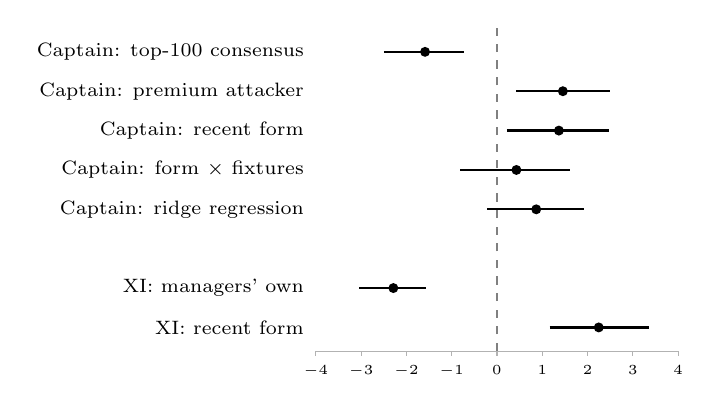
\begin{tikzpicture}[x=0.575cm,y=0.5cm]
\draw[gray!60] (-4,0.4) -- (4,0.4);
\foreach \x in {-4,-3,-2,-1,0,1,2,3,4} { \draw[gray!60] (\x,0.4) -- (\x,0.28) node[below,font=\tiny,text=black] {$\x$}; }
\draw[dashed,gray] (0,0.4) -- (0,8.60);
\node[anchor=east,font=\scriptsize] at (-4.05,8.00) {Captain: top-100 consensus};
\draw[thick] (-2.500,8.00) -- (-0.728,8.00); \fill (-1.588,8.00) circle (1.8pt);
\node[anchor=east,font=\scriptsize] at (-4.05,7.00) {Captain: premium attacker};
\draw[thick] (0.421,7.00) -- (2.491,7.00); \fill (1.456,7.00) circle (1.8pt);
\node[anchor=east,font=\scriptsize] at (-4.05,6.00) {Captain: recent form};
\draw[thick] (0.219,6.00) -- (2.483,6.00); \fill (1.368,6.00) circle (1.8pt);
\node[anchor=east,font=\scriptsize] at (-4.05,5.00) {Captain: form $\times$ fixtures};
\draw[thick] (-0.807,5.00) -- (1.623,5.00); \fill (0.430,5.00) circle (1.8pt);
\node[anchor=east,font=\scriptsize] at (-4.05,4.00) {Captain: ridge regression};
\draw[thick] (-0.211,4.00) -- (1.930,4.00); \fill (0.868,4.00) circle (1.8pt);
\node[anchor=east,font=\scriptsize] at (-4.05,2.00) {XI: managers' own};
\draw[thick] (-3.045,2.00) -- (-1.578,2.00); \fill (-2.288,2.00) circle (1.8pt);
\node[anchor=east,font=\scriptsize] at (-4.05,1.00) {XI: recent form};
\draw[thick] (1.162,1.00) -- (3.348,1.00); \fill (2.248,1.00) circle (1.8pt);
\end{tikzpicture}

\captionof{figure}{Model minus comparator, points per gameweek, with 95\% intervals over 114
gameweeks. Right of zero favours the model. XI comparisons use the top-100 managers' real squads.}
\end{minipage}

\begin{table}[h]
\centering\small
\begin{tabular}{lcc}
\toprule
 & Error (MAE) & Weekly rank$^*$ \\
\midrule
Model & \maeModel & \rhoCandModel \\
Ridge regression & \maeReg & \rhoCandReg \\
Recent form $\times$ fixtures & \maeFormScaled & \rhoCandForm \\
\bottomrule
\end{tabular}
\caption{Accuracy over \nTestRows{} player-weeks. $^*$Within-week rank correlation among regular
starters, the players managers actually choose between.}
\end{table}

\begin{itemize}
  \item \textbf{Forecasts: clearly better.} Lower error than every comparator and the best
        ranking of regular starters within each week.
  \item \textbf{Captains: better than naive rules only.} The model beats the priciest attacker
        by \vsPremiumMean{} points a week and unadjusted form by \vsFormMean{}. Against form scaled
        by fixtures (\vsFormScaled) and the regression (\vsReg) the difference is within noise.
        The edge over the price rule comes almost entirely from 2024/25.
  \item \textbf{Behind the best managers.} Their consensus captain outscores the model's by
        \gapElite{} points a week, and their elevens beat its picks too. So the model fails the
        pre-set rule.
  \item \textbf{Robust.} Ten variants with inputs removed or settings changed, plus a block
        bootstrap, give the same verdict.
\end{itemize}

\section{Why the best managers still win}
They know things the model does not: team news, late injuries, penalty duty
\citep{bonello2019}. The comparison also flatters them: they are in the sample \emph{because}
their season went well, a survivorship effect \citep{brown1992}.

\section{Usage rate, explained}
Basketball's usage rate is the share of a team's possessions a player ends while on the floor
\citep{bbrefglossary,oliver2004}. A football version \citep{sincerefc2025a,sincerefc2025b} counts
shots plus every lost ball. With Opta data \citep{plstats},
\[
  \text{usage}_i = 100\cdot\frac{\text{actions}_i\cdot(\text{team minutes}/11)}{\text{minutes}_i\cdot\text{team actions}}.
\]
It is a revealing chart of who needs the ball and who makes the most of it. As a predictor,
last season's usage cut forecast error by only \usageMaeGain{} points. Captain and lineup choices
did not change detectably.

\section{One lesson for anyone judging FPL advice}
Weekly captain scores are noisy: two captaincy rules' weekly difference has a standard deviation of
about 5 points. Measuring a one-point-a-week edge to $\pm1$ takes about 96 gameweeks. Reliably
detecting it takes about 196, five seasons. A good month proves very little.

\section{Takeaways for managers}
\begin{itemize}
  \item Minutes first. Recent minutes and starts matter more than any other input group.
  \item Count fixtures. Much of a model's apparent edge over simple form disappears once form is
        scaled for double gameweeks.
  \item Judge advice over seasons, not weeks.
\end{itemize}

\section{What happens next}
From gameweek 7 of 2026/27, the model's captain is logged before every deadline beside the official
expected-points pick and a price rule. Logs are frozen at the deadline and scored afterwards.

{\footnotesize
\setlength{\bibsep}{1pt}
\begin{thebibliography}{21}
\bibitem[Basketball-Reference(2026)]{bbrefglossary} Basketball-Reference. Glossary: usage percentage. \url{https://www.basketball-reference.com/about/glossary.html}.
\bibitem[Bonello et~al.(2019)]{bonello2019} N.~Bonello, J.~Beel, S.~Lawless, J.~Debattista. Multi-stream data analytics for enhanced performance prediction in fantasy football. \emph{AICS}, 284--292, 2019.
\bibitem[Brown et~al.(1992)]{brown1992} S.~J. Brown, W.~Goetzmann, R.~G. Ibbotson, S.~A. Ross. Survivorship bias in performance studies. \emph{Rev. Financ. Stud.} 5(4):553--580, 1992.
\bibitem[Dixon and Coles(1997)]{dixoncoles1997} M.~J. Dixon, S.~G. Coles. Modelling association football scores and inefficiencies in the football betting market. \emph{J. R. Stat. Soc. C} 46(2):265--280, 1997.
\bibitem[Efron and Tibshirani(1993)]{efron1993} B.~Efron, R.~J. Tibshirani. \emph{An Introduction to the Bootstrap}. Chapman \& Hall, 1993.
\bibitem[Fantasy Premier League(2026a)]{fplapi} Fantasy Premier League. Public data endpoints. \url{https://fantasy.premierleague.com/api/}.
\bibitem[Fantasy Premier League(2026b)]{fplrules} Fantasy Premier League. Rules. \url{https://fantasy.premierleague.com/help/rules}.
\bibitem[Frees et~al.(2024)]{frees2024} D.~Frees, P.~Ravella, C.~Zhang. Deep learning and transfer learning architectures for English Premier League player performance forecasting. arXiv:2405.02412, 2024.
\bibitem[Friedman(2001)]{friedman2001} J.~H. Friedman. Greedy function approximation: a gradient boosting machine. \emph{Ann. Stat.} 29(5):1189--1232, 2001.
\bibitem[Gupta(2019)]{gupta2019} A.~Gupta. Time series modeling for dream team in Fantasy Premier League. arXiv:1909.12938, 2019.
\bibitem[Lombu et~al.(2024)]{lombu2024} A.~S. Lombu, I.~V. Paputungan, C.~K. Dewa. Predicting Fantasy Premier League points using CNN and LSTM. \emph{JUTIF} 5(1):263--272, 2024.
\bibitem[Maher(1982)]{maher1982} M.~J. Maher. Modelling association football scores. \emph{Stat. Neerl.} 36(3):109--118, 1982.
\bibitem[Nosek et~al.(2018)]{nosek2018} B.~A. Nosek, C.~R. Ebersole, A.~C. DeHaven, D.~T. Mellor. The preregistration revolution. \emph{PNAS} 115(11):2600--2606, 2018.
\bibitem[Oliver(2004)]{oliver2004} D.~Oliver. \emph{Basketball on Paper}. Potomac Books, 2004.
\bibitem[Premier League(2026)]{plstats} Premier League. Player and club statistics (Opta data). \url{https://www.premierleague.com/stats}.
\bibitem[Ramezani and Dinh(2025)]{ramezani2025} D.~Ramezani, T.~Dinh. A data-driven framework for team selection in Fantasy Premier League. arXiv:2505.02170 (v3), 2025.
\bibitem[Sincere FC(2025a)]{sincerefc2025a} Sincere FC. The NBA stat that could change football. YouTube, 2025. \url{https://www.youtube.com/watch?v=iydcB3OM6EE}.
\bibitem[Sincere FC(2025b)]{sincerefc2025b} Sincere FC. The NBA stat that explains football transfers. YouTube, 2025. \url{https://www.youtube.com/watch?v=-Ga-oiyM0aQ}.
\bibitem[Tashman(2000)]{tashman2000} L.~J. Tashman. Out-of-sample tests of forecasting accuracy: an analysis and review. \emph{Int. J. Forecast.} 16(4):437--450, 2000.
\end{thebibliography}
}

\end{document}
